\documentclass[12pt,a4paper]{article}
\usepackage[a4paper,left=3cm,right=2cm,top=3cm,bottom=2cm]{geometry}
\usepackage[brazil]{babel}
\usepackage{iftex}

\ifPDFTeX
    \usepackage[T1]{fontenc}
    \usepackage[utf8]{inputenc}
    \usepackage[scaled=0.95]{helvet}
    \renewcommand{\familydefault}{\sfdefault}
\else
    \usepackage{fontspec}
    \setmainfont{Arial}
\fi

% Core packages
\usepackage{amsmath,amssymb}
\usepackage{tikz-cd}
\usepackage{multicol}
\usepackage{setspace}
\usepackage{xurl}
\usepackage{url}
\usepackage{acronym}
% Paragraphs
\onehalfspacing
\setlength{\parindent}{1.25cm}
\setlength{\parskip}{0pt}
\usepackage{float}
\acrodef{AGV}{Automated Guided Vehicles}
\acrodef{MD}{Manhattan Distance}

\title{Planejamento de Rotas de AGVs em Centro de Distribuição Automatizado}
\date{\today}
\author{Alan de Queiroz da Silva, Alysson dos Anjos de Oliveira da Costa, \\Cainan Brito Araujo Santos,Letícia Costa Oliveira Almeida}


\begin{document} 
\maketitle

\section{Introdução}

Este trabalho apresenta o desenvolvimento de um agente inteligente para planejamento de rotas de veículos autônomos guiados, os chamados AGVs, do inglês \textit{Autonomous Guided Vehicles}, em um centro de distribuição automatizado, aplicando conceitos de modelagem de agentes solucionadores de problemas e busca em espaço de estados. Serão analisados algoritmos como Busca em largura, Busca em profundidade, Busca de custo uniforme, Busca Gulosa e A*, considerando obstáculos, restrições operacionais e custos de movimentação, além da utilização da especificação PEAS e de funções heurísticas para otimização das rotas. Ao final, será realizada uma comparação de desempenho entre os algoritmos, avaliando eficiência, custo e tempo de processamento.

\section{Contexto}

Centros de distribuição modernos dependem cada vez mais de veículos autônomos guiados, para movimentar mercadorias entre áreas de armazenamento, separação e expedição. Em operações desse tipo, atrasos, gargalos e escolhas ruins de rota podem comprometer a produtividade de todo o sistema logístico.

O ambiente interno de um centro de distribuição não é homogêneo nem previsível. Diversos trechos podem apresentar corredores estreitos com sentido único de circulação, cruzamentos de alta circulação com custos maiores de travessia, áreas de reabastecimento, bloqueios temporários que podem invalidar rotas já planejadas, entre outros. Estes fatores tornam insuficiente uma abordagem ingênua de planejamento, exigindo um agente capaz de avaliar alternativas e 
selecionar a rota que melhor atenda aos critérios operacionais do armazém.

\section{Especificação PEAS do agente}

Para tornar a especificação do agente mais clara, o problema pode ser descrito segundo o modelo PEAS (\textit{Performance, Environment, Actuators, Sensors}), conforme a seguir.

\begin{description}
    \item[Performance (desempenho)] ~\\
    \begin{itemize}
        \item Minimizar o tempo total necessário para transportar uma mercadoria até a área de destino;
        \item Reduzir o consumo de energia ou combustível durante o trajeto;
        \item Evitar danos ao veículo e à carga transportada;
        \item Evitar obstáculos e áreas restritas do ambiente; e
        \item Respeitar regras de deslocamento e tráfego interno, com redução do risco de acidentes e atrasos.
    \end{itemize}

    \item[Environment (ambiente)] ~\\
    \begin{itemize}
        \item Centro de distribuição com tráfego controlado e regras específicas de circulação representadas em um grid ou grafo;
        \item Ambiente dinâmico, em que bloqueios, congestionamentos e áreas interditadas podem surgir ao longo do percurso;
        \item Presença de diferentes custos de deslocamento entre regiões do ambiente;
        \item \textbf{Parcialmente observável}: o \ac{AGV} possui percepção limitada pelos sensores embarcados;
        \item \textbf{Estocástico}: Pois imprevistos podem alterar estados, ações disponíveis e custos de trajeto. Em ambientes estocásticos o próximo estádo do mesmo não é definido pela movimentação do agente, ou seja, uma mesma ação pode levar a resultados diferentes.  \cite{russell2021};
        \item \textbf{Sequencial}: cada decisão de rota influencia as decisões futuras;
        \item \textbf{Dinâmico}: o ambiente pode mudar enquanto o agente executa a rota;
        \item \textbf{Contínuo}: o tempo de execução e as condições operacionais variam durante a ação; e
        \item \textbf{Multiagente}: há múltiplos \ac{AGV} compartilhando o mesmo espaço logístico.
    \end{itemize}

    \item[Actuators (atuadores)] ~\\
    \begin{itemize}
        \item Sistema de direção para movimentação nas quatro direções possíveis;
        \item Sistema de aceleração e frenagem;
        \item Sistema de controle de rota para recalcular o percurso quando necessário;
        \item Sistema de luzes e sinais sonoros para indicar chegada ao destino ou alertas operacionais; e
        \item Sistema de sinalização direcional para informar a próxima manobra.
    \end{itemize}

    \item[Sensors (sensores)] ~\\
\begin{itemize}
        \item Sensores de velocidade para monitorar e limitar a velocidade máxima;
        \item Câmeras para observar o ambiente, detectar imprevistos e identificar regras de tráfego, como sentido único e limite de velocidade;
        \item Sensor de proximidade para evitar colisões com obstáculos ou outros veículos;
        \item Sensor de localização para determinar a posição do \ac{AGV} no grid;
        \item Sensor de peso para verificar se a carga está dentro da capacidade máxima e auxiliar na escolha da rota e da velocidade adequadas, auxiliando também na decisão do veículo ao subir rampas ou fazer curvas muito fechadas;
        \item Sistema de comunicação entre \ac{AGV}s, permitindo troca de dados e coordenação operacional.
    \end{itemize}
\end{description}


\section{Modelagem do problema de busca}

A modelagem do problema de busca representa o ambiente logístico como um espaço discreto, no qual o \ac{AGV} deve sair de uma posição inicial, coletar uma carga, entregá-la no destino correto e, ao final da tarefa, retornar a um ponto de repouso ou aguardar uma nova instrução.

\subsection{Estado inicial}

O estado inicial não necessariamente é o estado onde o pacote está disponível para coleta. Ele corresponde ao \ac{AGV} parado na área de estacionamento ou no local de armazenamento dos veículos, sem carga e disponível para receber uma nova tarefa. 

\subsection{Representação dos estados}

Cada estado pode ser descrito por um conjunto de atributos relevantes para a tomada de decisão:

\begin{itemize}
    \item Posição do \ac{AGV} no grid, representada por coordenadas $(x, y)$;
    \item Condição de operação do veículo, como \textit{em repouso}, \textit{em trânsito para coleta} ou \textit{em trânsito para entrega};
    \item Existência ou não de carga transportada;
    \item Custo acumulado do percurso até o estado atual;
    \item Presença de bloqueios, obstáculos temporários ou restrições no entorno imediato;
    \item Se o pacote possui prioridade de entrega;
    \item Se o veículo esta com sobrepeso
\end{itemize}


De forma mais específica, o \ac{AGV} pode assumir status de estados operacionais como:

\begin{itemize}
    \item \textbf{Em repouso}: Aguardando uma nova tarefa;
    \item \textbf{Coletando}: Percorrendo o caminho até o ponto de coleta dos pacotes;
    \item \textbf{Entregando}: Percorrendo o caminho até a doca de expedição ou ponto de entrega.
\end{itemize}

\subsection{Objetivos}

Os objetivos do agente no problema de busca são:

\begin{itemize}
    \item Alcançar o ponto de coleta dos pacotes;
    \item Transportar a carga até um ou mais pontos de entrega;
    \item Após concluir a tarefa, retornar ao ponto de descanso ou ao estado inicial.
\end{itemize}

\subsection{Operadores ou ações}

As ações disponíveis ao \ac{AGV} modificam seu estado no ambiente e possuem custo associado, seja em tempo, energia ou risco operacional. Entre as principais ações, destacam-se:

\begin{itemize}
    \item Movimentar-se no ambiente nas direções permitidas pelo modelo adotado;
    \item Acelerar;
    \item Frear;
    \item Aguardar, quando houver bloqueio temporário ou necessidade de parada;
    \item Coletar pacote(s);
    \item Entregar pacote(s).
\end{itemize}

\subsection{Modelo de transição}

As transições entre estados ocorrem de acordo com as ações executadas e com as condições observadas no ambiente:

\begin{itemize}
    \item Ao coletar um pacote, o \ac{AGV} passa a executar a rota até o ponto de entrega correspondente;
    \item Ao concluir uma entrega, caso ainda existam pacotes pendentes, o agente continua a operação de entrega ou segue para a próxima coleta;
    \item Se a entrega concluída for a última da tarefa, o \ac{AGV} retorna ao estado inicial ou ao ponto de descanso;
    \item Ao tentar mover-se para um espaço livre, o \ac{AGV} assume uma nova posição $(x, y)$ e atualiza o custo acumulado;
    \item Ao tentar mover-se para um espaço comprometido, como uma área interditada ou ocupada por obstáculo fixo ou dinâmico, a ação é considerada inválida.
\end{itemize}

No caso da ação de espera, o comportamento do agente pode ser definido da seguinte forma:

\begin{itemize}
    \item Se houver um obstáculo dinâmico ou temporário à frente, o \ac{AGV} permanece aguardando;
    \item Se o obstáculo persistir por tempo superior a um limite predefinido, ele pode ser tratado como bloqueio fixo para fins de replanejamento;
    \item Se houver obstáculo fixo, o agente recalcula a rota; e
    \item Se o caminho voltar a ficar livre, o \ac{AGV} retorna ao estado operacional anterior e prossegue com a tarefa.
\end{itemize}

\subsection{Custo do Caminho}
\section{Heurística e algoritmos de busca}
A heurística adotada na implementação do sistema foi a \ac{MD}, por ser uma medida amplamente utilizada em problemas de busca em grade . Essa heurística é adequada para cenários em que o agente se movimenta em quatro direções: cima, baixo, direita e esquerda, pois estima o custo até o objetivo com base na soma das diferenças horizontais e verticais entre a posição atual e a posição de destino \cite{patelheuristics}. Essa heurística é considerada admissível nesse tipo de problema, por nunca superestimar o custo para chegar ao seu objetivo.

\begin{figure}[H]
    \centering
    
    \includegraphics[scale=.5]{manhattan.png}
    \caption{Imagem representando movimentação \ac{MD} em um ambiente qualquer}
    \label{table:depth}
\end{figure}

O pseudocódigo da implementação da heurística utilizada pode ser descrito da seguinte forma:

\begin{minipage}{0.7\textwidth}
\centering
\begin{verbatim}

 D * (abs(x - x2) + abs(y - y2)) 

\end{verbatim}
\end{minipage}
\begin{itemize}
    \item D: Representa o menor custo de movimento
    \item Abs: É uma função matemática para retornar o valor absoluto do resultado
    \item X e Y: Representam a posição atual do \ac{AGV} dentro do grid
    \item X2 e Y2: Representam a posição do objetivo dentro do grid
\end{itemize}

Nesse sentido, para melhor visibilidade dos resultados, as múltiplas instâncias foram avaliadas de forma comparativa em diferentes algoritmos:
\begin{itemize}
    \item \textbf{Busca em largura:} Explora os todos os nós de um nivel antes de partir para o próximo, utiliza uma fila (FIFO) para saber quais os nós que foram visitados, previnindo loops infinitos e uso excessivo de memória \cite{mediumsearch} \cite{geeksforgeekssearch}

    \item \textbf{Busca em profundidade:} Explora o máximo possível cada caminho antes de realizar retorno \textit{backtracking}. Utiliza uma pilha (LIFO) e possue maior eficiencia em termos de memória do que a busca em largura, porém não garante encontrar o caminho mais curto. \cite{mediumsearch} \cite{geeksforgeekssearch}
    
    \item \textbf{Busca de custo uniforme:} É uma extensão do método de busca em largura, porém considerando o custo do caminho, expandingo sempre o nó de menor custo primeiro \cite{geeksforgeekssearch}

    \item \textbf{Busca Gulosa:} Segue uma abordagem orientada a objetivo,sempre expandindo um nó que aparenta estar mais próxima da meta com base em uma estimativa heurística.O algoritmo é chamado de guloso porque prioriza ganhos imediatos sem considerar o custo total do caminho. \cite{mediumsearch}
    
    \item \textbf{A*:} È uma combinação dos melhores aspectos da busca gulosa e dos algoritmos de busca de custo uniforme, utilizando tanto o custo do caminho quanto informações heurísticas \textbf{(f(n) = g(n) + h(n))}, para encontrar uma solução eficiente e ótima.\cite{mediumsearch}
\end{itemize}

\section{Descrição da implementação}
A implementação foi desenvolvida no editor de código \textit{Visual Studio Code}, utilizando a linguagem Python e a biblioteca SimpleAI para a construção das rotinas de busca e para o tratamento de funcionalidades relacionadas à inteligência artificial.

\begin{figure}[H]
    \centering
    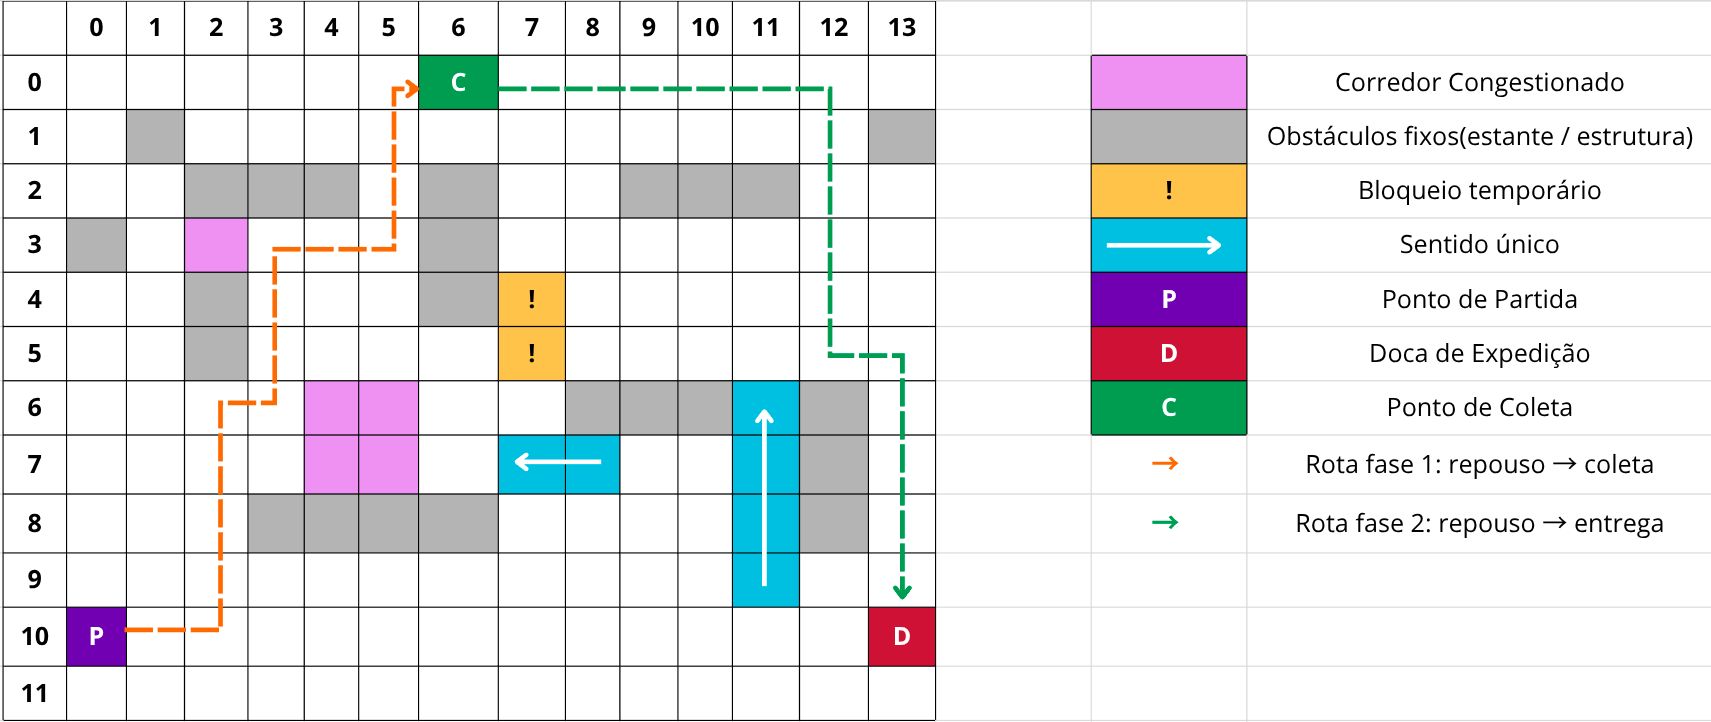
\includegraphics[scale=.25]{fluxo-agv.png}
    \caption{Representação do Mapa do Armazém em grid}
    \label{table:depth}
\end{figure}



\section{Resultados e análise comparativa}

\section{Conclusão}


\nocite{*}
\bibliographystyle{plain}
\bibliography{referencias}

\section{Prompts utilizados}

\end{document}
